\chapter{DISCUSSION \& ANALYSIS}
\section{Introduction}
After clarifying the data collection process and the relevant procedures adopted for
the analysis, this chapter aims to examine the previously collected data in order to determine
the definitive truth regarding hressing AI into higher education. To this end, statistical
tables and graphs would be disclosed. The findings of this
paper are consistent with previous research results on the practical ways of implementing AI into
humanities, students' point of view about their preformance while using AI, challanges and oppurtunites.
In short, the survey’s results indicate that students academic performance is improved while using AI.
\section{Results}
% In this sections, a descriptive statistic technique was used to
% interpret the data collected from English
% university students through filling out Google form.
The data collected from the survey conducted among English university students
revealed compelling insights into the students' perceptions and experiences with AI-driven tools.
The analysis utilized descriptive statistical techniques to interpret the responses gathered through the questionnaire.
The questionnair divided into two main parts: the first part is to investigate
whether the students' academic performance have improved or not while using AI-driven. The second
part is about challenges and oportunites faced during using AI for academic studies.

\subsection{The students' academic performance while using AI-driven tools}
\begin{figure}[h]
	\centering
	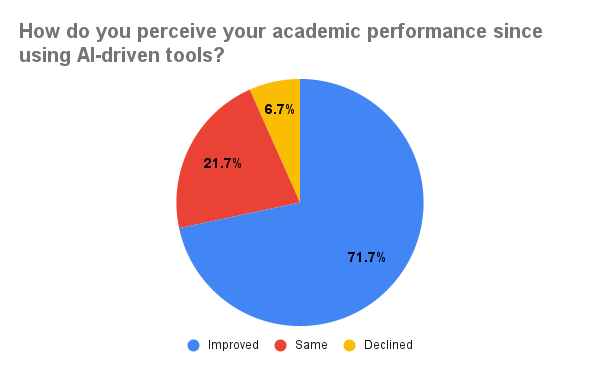
\includegraphics[width=11cm, height=7cm]{./chap4/figures/prf}
	\captionof{figure}{perceive academic performance using AI-driven tools}
\end{figure}
After assessing the respondents’ opinions on the use of AI-driven tools
and students' academic preformance, it is obvious that the majority
of their academic preformance was improved. it is clearly shown that
74.3\% agreed that AI improve their academic performance. In addition to
20\% of respondents believed that the use of AI didn't affect their academic
performance. Whereas 4.7\% showed their negative resulte believing that AI
affect their academic preformance to be declined while using it.

\subsection{The students' engagments while using AI-driven tools in academic setting}

\begin{figure}[H]
	\centering
	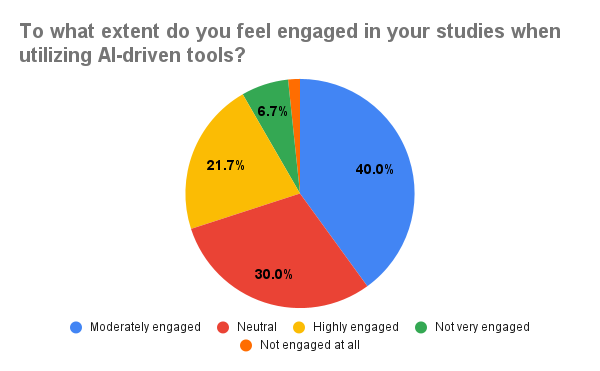
\includegraphics[width=11cm, height=7cm]{./chap4/figures/engagment}
	\captionof{figure}{perceive academic engagment using AI-driven tools}
\end{figure}

The data collected on the extent of students engagement when using AI-driven tools
provides a diverse range of percaptions and experiences. While a significant portion
of respondents reported moderate engagment 34.8\%, indicating a level of engagment with
these AI-driven tools, an almost equal of neuturality 34\%, suggesting a mixed reception.
However, a notable subset of students reported feeling highly engaged 20.8\%, depicting that
these tools can effectively encourage students to be engaged. Negatively, the presence
of respondents feeling not very engaged 7.5\% or not engaged at all \% highlights potential
limitations or challenges associated with the implementation or usage of AI-driven tools.


\subsection{Challenges faced while using AI-driven tools in academic setting}

\begin{figure}[H]
	\centering
	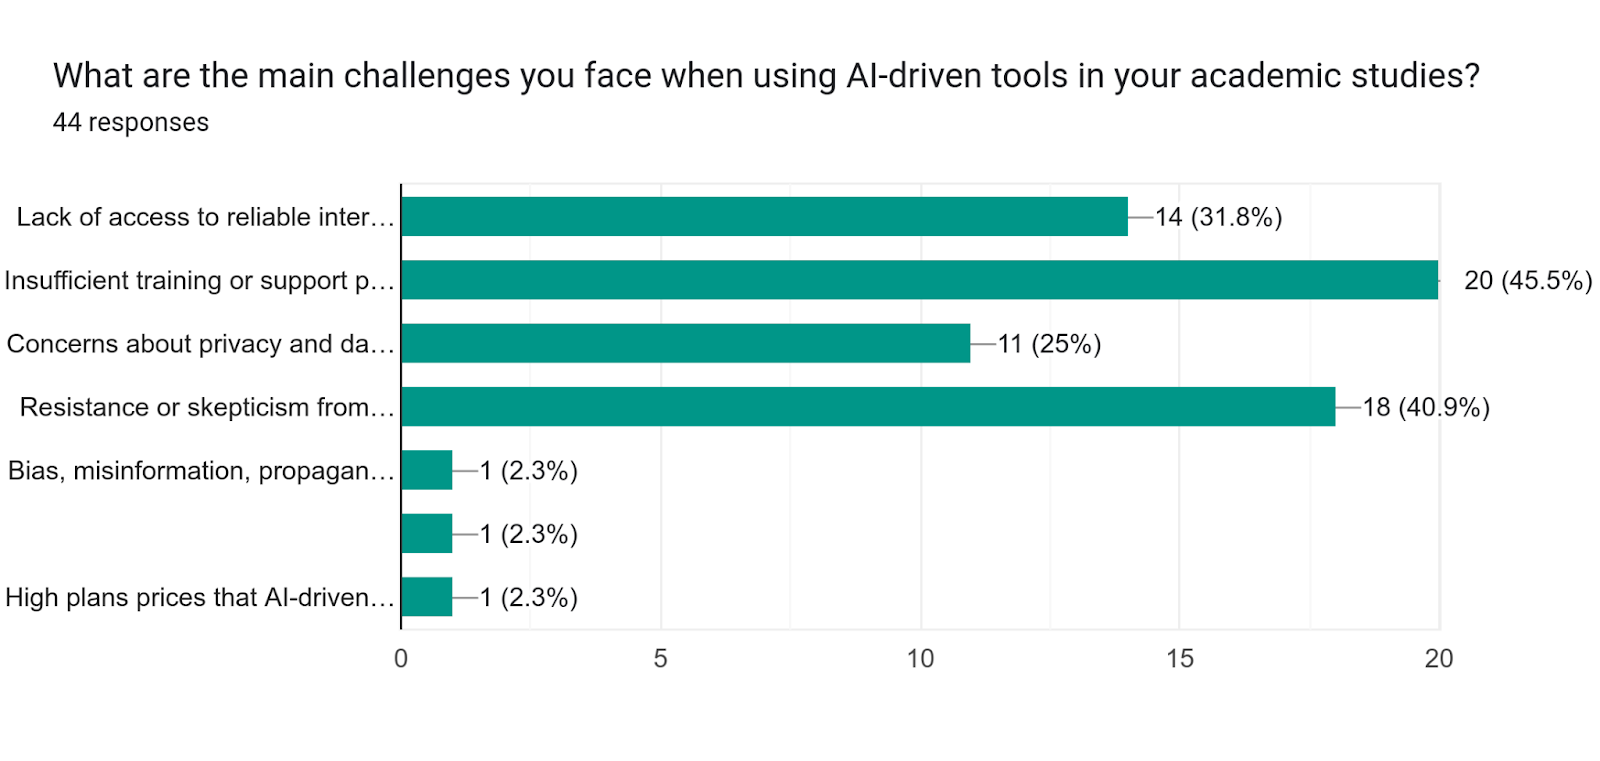
\includegraphics[width=17cm, height=9cm]{./chap4/figures/chall}
	\captionof{figure}{challenges faced when using AI-driven tools in academic setting}
\end{figure}

The bar chart shows the results of a survey on the challenges students
face when using AI-driven tools in their academic studies. Out of 44 respondents,
the biggest challenge was reported to be insufficient trainging for these
tools, with 45.5\% of students selecting this options. While resistance or skepticism
from professors towards using AI-driven tools was reported to be the second challenge
face by students with 40.9\%.
Following this was lack of access to reliable internet, with 31.8\% of students
reporting this as a challenge.
A smaller percentage of students reported facing challenges with pricacy and data security matters
with 25\%. while 2.3\% was bias, misinformation, propaganda in the AI tools and high prices of the AI-driven tools.

% The blow bar chart has shown that 45.5\% of English university
% students face Insufficient training
% as main challenge. In addition 40.9\% was resistance
% or skepticism from professors towards using AI-driven tools in
% academic settings. While 31.8\% and
% 25\% were lack of access to relaible internet and privacy comcerns. whereas
% 2.3\% was bais and high plans prices that AI-driven tools offer.
\subsection{AI-driven tools and opportunities for improving learning experiences in the humanities }
\begin{figure}[H]
	\centering
	\captionof{figure}{AI-driven tools and oppu}
	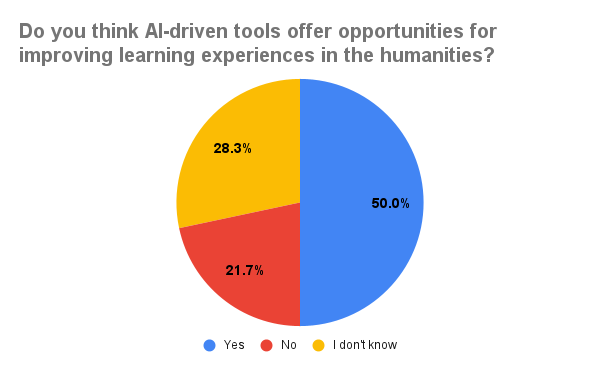
\includegraphics[width=11cm, height=7cm]{./chap4/figures/op.png}
\end{figure}

The majority of English university students reported with 50.9\% that AI-driven tools offer opportuinities
for enhancing learning experiences in the humanities. In addition to 28.9\% to report the
ignorance of the opportunities that AI-driven tools offer. Whereas 20.8\% negatively reported
the idea of AI-driven tools offers such opportunity for enhancing the learning experience
within humanities setting.


Those who answered with yes a question is asked to get some examples from students
to understand what kind of opportunities AI-driven tools can offer to enhance the learning experiences and answers were follow:

% 1st resp
\resp{1}{AI-driven tools in higher education could enhance personalized learning
	through adaptive learning platforms and virtual
	tutoring, and improve research with data analysis tools.}
% 2nd resp
\resp{2}{Research Assistance: AI can assist
	researchers in analyzing vast amounts of
	data, generating hypotheses, and identifying trends,
	accelerating the pace of discovery.}
% 3rd resp
\resp{3}{It can help students be more self-reliant
	and seek knowledge wherever and whenever they want to.}
%4rd resp 
\resp{4}{Making student more used to communicate with chat
	bot ai characters when they can't find native speakers to communicate with.}
%5th resp
\resp{5}{It helps you correct some mistakes and learn from them. 
It elevates your writing and information base and limit their context.}

As it is shown the majority of english students to claim that AI-driven tools can
help students to boost their productivity through analysing the data for researcheres
and provide personalized learning through adaptive learning platforms and virtual tutoring.

\section{Discussion}
It would be more fitting to restate the current study’s goals and research hypothesis
before digging deeper into the research findings and discussion. As mentioned in the
introduction, the main objective of this paper is to evaluate English students’ attitudes towards the
use of AI-driven tools for enhancing their academic prefromance and learning experiences.
learners. Accordingly, the recent study has significantly helped
to validate or reject the hypotheses stated in the previous chapter.
These later were formed as follows:
\begin{itemize}
	\item AI-driven tools are singificantly fostering engagment in academic setting.
	\item AI-driven tools are significantly improving academic performance.
	\item There are challenges and opportunities are associated with using AI in higher education
	      in Morocco, specifically in the humanities
\end{itemize}
The current study’s findings strongly demonstrate positive attitudes by students towards
the use AI-driven tools as learning tool. The students have been asked precise questions
to explore their perceptions on the use of AI-driven tools

Firstly, the findings reveal a notable increase in student engagement 37\% when 
utilizing AI technologies. The data collected from English university students
strongly supports the idea that AI can effectively enhance student engagement,
fostering a more interactive and dynamic learning environment. This aligns with
existing literature that emphasizes the role of technology in promoting active
participation among students.

Secondly, the research results demonstrate a positive correlation between the use of AI-driven tools and students' academic performance. 
As data results reveal, the major part of participants 74\% believed that AI-driven tools
improved their academic performance. In the same way, 
\citep{mohammed_exploring_2023} performed a related study
to demonstrate that AI-driven tools can effectively enhance 
academic preformance and foster engagment. Results showed
that the majority of respondents agreed that \say{ChatGPT} 
motivates and engages students by offering access to 
many resources and improving academic perormance. 

% Based on the findings, majority of respondents showed great eagerness using
% AI-driven tools that helps them to enhance their academic preformance and engagment.
% The responses were positive as only 4 participants out of 53 AI does not take a place
% enhacing their learning experiences.
Furthermore, the research findings shed light on the challenges encountered by 
students when utilizing AI-driven tools in educational settings. These challenges,
as reported by the participants, offer valuable insights into the practical obstacles
associated with the implementation of AI technologies in learning environments.
Issues such as technical difficulties, lack of training, resistance or skipticism of professors, 
and concerns regarding data privacy and security emerge as significant 
hurdles that need to be addressed to ensure the effective utilization of AI in education.


Lastly, the research results highlight the opportunities presented by AI-driven 
tools for transforming learning experiences in the humanities. By exploring 
students' perspectives and experiences with AI technologies, the study uncovers 
the potential for personalized learning, adaptive tutoring, and data analysis to help researchers
with their vas-amount data. These opportunities align with the broader literature 
on the transformative impact of AI in education, emphasizing the role of technology 
in facilitating innovative and tailored learning experiences. Leveraging these 
opportunities can empower educators to create engaging, effective, and personalized 
learning environments that cater to the diverse needs of students in the humanities.

% The usage of AI-driven tools face many challanges majorty of English students
% reported that insufficient training for using AI-driven tools to be one of the challenges faced.
% While resistance or skipticism of professors is also a challenge for not taking advantage of these
% tools to enhance their learning experiences. Wherase the lack of accessing to relaible internet and
% the pravicy concerns to be less payed attention. The AI-driven tools are not only offering challenges
% but also opportunities. 50\% of English students to report that AI-driven tools offers a vast oppurtonities 
% such as personalized learning, data analytics to help researchers analysis their data, and a way for improving
% ones' English. 

\section{Conclusion}
Throughout this chapter, we have conducted an ongoing study related to students’
attitudes towards the use of AI-driven tools as a learning tool to enhance the learning experiences
within academic setting. The aim was to present and discuss the findings of the study in depth.
Additionally, this study sought to validate or reject the formulated hypotheses mentioned
in the methodology chapter, and correlate the concluded findings with the paper’s literature
review and see how far it converges or diverges from it. The final chapter would discuss
the implications and the limitations of this study. Finally, it will cover an inclusive summary
of the research paper and serve as a springboard to a more in-depth analysis.
